The algorithms are used to solve VPGs created from different test cases. We have two model checking problems as well as random VPGs. The model checking VPGs are created as described in part \ref{part:verifying}, with the exception that only vertices are added when they are reachable from the initial vertex. So these games are never disjointed, random games can be disjointed.

\subsection{Model checking games}
We use two software product line examples, first the minepump example as described in \cite{Kramer1983CONICAI} and implemented in the mCRL2 toolset as described in \cite{FamBasedModelCheckingWithMCRL2}. The minepump example models the behaviour of controllers for a pump that pumps water out of a mineshaft. There are 10 different features that change the way the sensors/actors behave. In total there are 128 valid feature assignments, i.e. products. 

The mCRL2 implementation creates an LTS with parametrized actions, the parameters describe the boolean formula's guarding the transitions, effectively making it an FTS. This FTS is interpreted in combination with nine different $\mu$-calculus formula's to create nine VPGs. The model uses 10 features, however only 128 feature assignments are valid. The FTS consists of 582 states and 1376 transitions. The resulting VPGs have on average 6600 vertices per game. Note that our implementation still creates BDDs using 10 boolean variables even though 7 would be enough to represent 128 configurations. By using the same number of variables as there are features the boolean formula's from the FTS are left intact when using them in the VPG.

Next we have the elevator example, described in \cite{PLATH200153}. This example models the behaviour of an elevator where five different features modify the behaviour of the model. All feature assignments are valid. Therefore we have $2^5 = 32$ feature assignments, i.e. products. Again an mCRL2 implementation\footnote{\label{note1}https://github.com/SjefvanLoo/VariabilityParityGames/blob/master/implementation/Elevator.tar.gz} (created by T.A.C. Willemse) is used to create seven VPGs. The FTS consists 95591 states and 622265 transitions. The resulting VPGs have on average 3659210 vertices per game. 
\subsection{Random games}
Random VPGs can be created by creating a random parity game and create sets of configurations that guard the edges. For these sets we need to consider two factors: how large are the sets guarding the edges and how are they constructed.

The guard sets in the minepump and elevator games have a very specific distribution where nearly all of the sets admit either $100\%$ or $50\%$ of the configurations. This is because an edge requiring the presence or absence of one specific feature results in a set admitting $50\%$. On average the edges in the examples admit $92\%$ of the configurations. Most likely VPGs originating from FTSs will have such a distribution.

We use $\lambda$ to denote the average relative size of guard sets in a VPG. So for every guard set in a VPG we divide its size by the total number of configurations to get the relative size of the guard set. Taking the average of all these relative sizes calculates $\lambda$.

We create a random game with a specific $\lambda$ by using a probabilistic distribution ranging from $0$ to $1$ to determine the size of an individual guard set. Such a distribution must have a mean equal to $\lambda$. We consider two distributions:
\begin{itemize}
	\item A modified Bernoulli distribution; in a Bernoulli distribution there is a probability of $p$ to get an outcome of $1$ and a probability of $1-p$ to get an outcome of $0$. We modify this such that there is a probability of $p$ to get $1$ and a probability of $1-p$ to get $0.5$. This gives a mean of $1p + 0.5(1-p) = 0.5p + 0.5$. So to get a mean of $\lambda$ we choose $p = 2\lambda - 1$. Note that we cannot use this distribution when $\lambda < 0.5$ because $p$ becomes less than $0$.
	\item A beta distribution; a beta distribution ranges from $0$ to $1$ and is curved such that it has a specific mean. The beta distribution has two parameters: $\alpha$ and $\beta$ and a mean of $\frac{\alpha}{\alpha+\beta}$. We pick $\beta=1$ and $\alpha = \frac{\lambda\beta}{1-\lambda}$ to get a mean of $\lambda$.
\end{itemize}
Figures \ref{fig:dist_lambda50}, \ref{fig:dist_lambda75} and \ref{fig:dist_lambda90} show the shapes of the distribution for different values for $\lambda$.
\begin{figure}[H]
	\centering
	\begin{subfigure}{.5\textwidth}
		\centering
		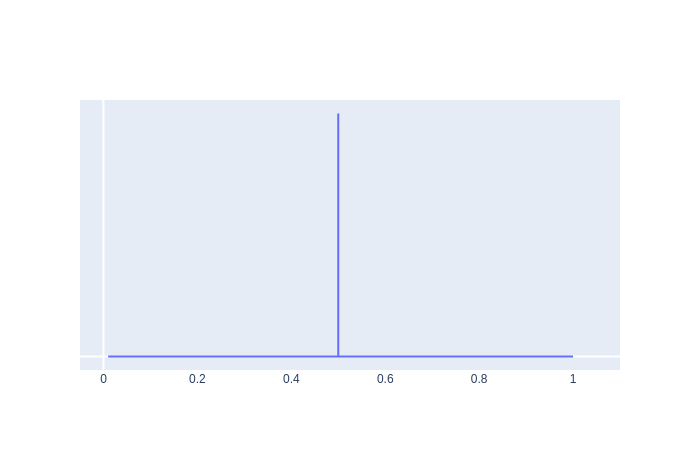
\includegraphics[width=\linewidth]{Dists/Bernoulli50.png}
		\caption{Modified Bernoulli distribution with $p=0$}
	\end{subfigure}%
	\begin{subfigure}{.5\textwidth}
		\centering
		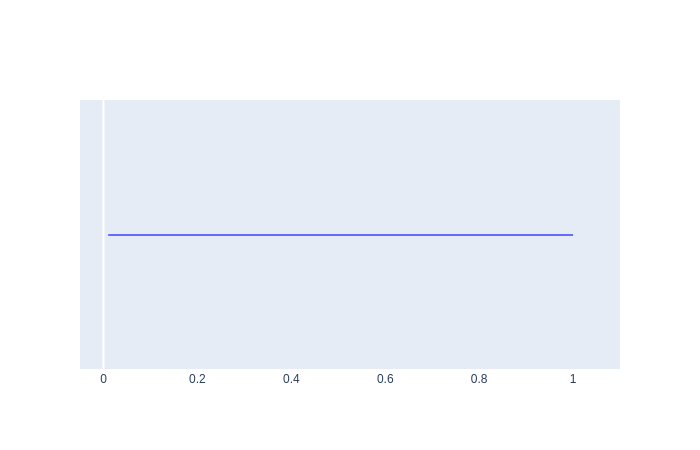
\includegraphics[width=\linewidth]{Dists/Beta50.png}
		\caption{Beta distribution with $\beta=1$ and $\alpha=1$}
	\end{subfigure}
	\caption{Edge guard size distribution for $\lambda = 0.5$}
	\label{fig:dist_lambda50}
\end{figure}%
\begin{figure}[H]
\centering
\begin{subfigure}{.5\textwidth}
	\centering
	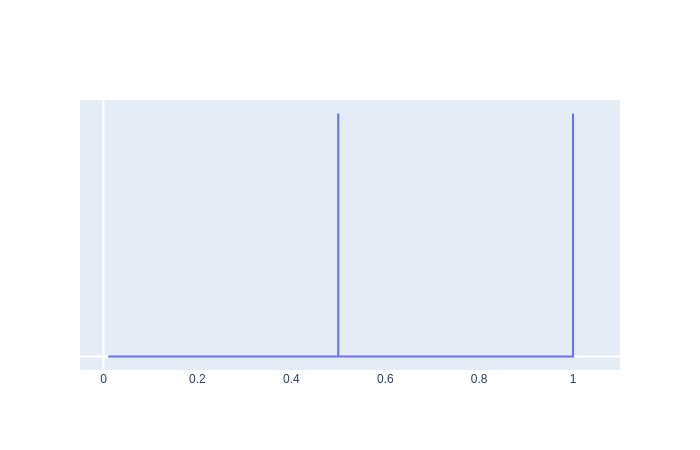
\includegraphics[width=\linewidth]{Dists/Bernoulli75.png}
	\caption{Modified Bernoulli distribution with $p=0.5$}
\end{subfigure}%
\begin{subfigure}{.5\textwidth}
	\centering
	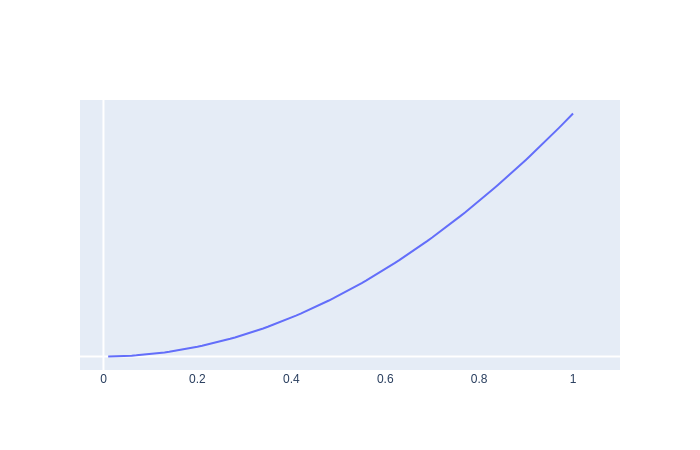
\includegraphics[width=\linewidth]{Dists/Beta75.png}
	\caption{Beta distribution with $\beta=1$ and $\alpha=3$}
\end{subfigure}
\caption{Edge guard size distribution for $\lambda = 0.75$}
\label{fig:dist_lambda75}
\end{figure}%
\begin{figure}[H]
\centering
\begin{subfigure}{.5\textwidth}
	\centering
	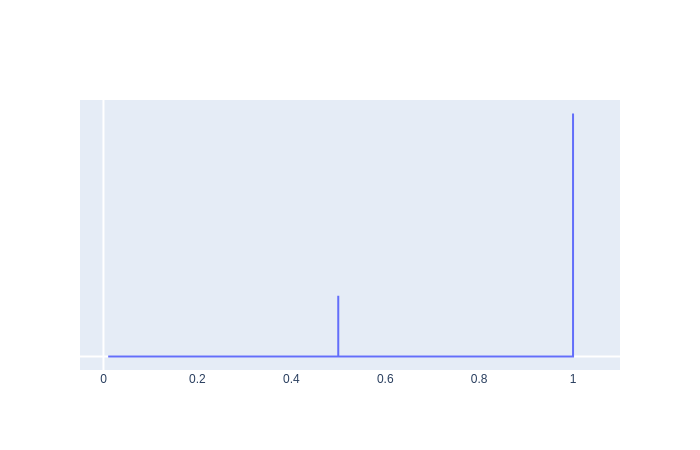
\includegraphics[width=\linewidth]{Dists/Bernoulli90.png}
	\caption{Modified Bernoulli distribution with $p=0.8$}
\end{subfigure}%
\begin{subfigure}{.5\textwidth}
	\centering
	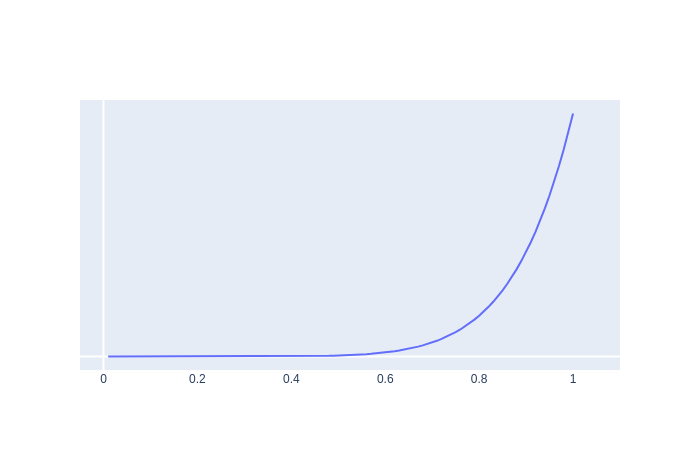
\includegraphics[width=\linewidth]{Dists/Beta90.png}
	\caption{Beta distribution with $\beta=1$ and $\alpha=9$}
\end{subfigure}
\caption{Edge guard size distribution for $\lambda = 0.9$}
\label{fig:dist_lambda90}
\end{figure}

Once we have determined the size for a configuration set we need to consider how the set is constructed. We can simply create a random set of configurations without any notion of features, we call this a \textit{configuration based} approach. Alternatively we can use a \textit{feature based} approach where we create sets by looking at features. Consider features $f_0, \dots, f_m$, we can create a boolean function that is the conjunction of $k$ features where every feature in the conjunction has probability $0.5$ of being negated.  For example when using $k=3$ and $m=5$ we might get boolean formula $f_1 \wedge \neg f_2 \wedge \neg f_4$. Such a boolean formula corresponds to a set of configurations of size $2^{m-k}$ and a relative size $\frac{2^{m-k}}{2^m} = 2^{-k}$, so when creating a set with relative size $r$ we choose $k = \min(m, \lfloor -\log_2{r} \rfloor)$. When using a feature based approach we can only create sets that have a relative size of $\frac{1}{2^i}$ for some $i \in \mathbb{N}$.

We can create 4 types of games:
\begin{enumerate}
	\item Bernoulli distributed and feature based. These games are most similar to the model verification games.
	\item Bernoulli distributed and configuration based. These games do have the characteristics of a model verification game in terms of set size but have unstructured sets guarding the edges. Furthermore with a configuration based approach less guard sets will be identical than with a feature based approach.
	\item Beta distributed and configuration based. These games are most different from the model verification games.
	\item Beta distributed and feature based. Games created in this way do not have the average relative set size of $\lambda$ because the feature based approach can only create sets of size $\frac{1}{2^i}$ for any $\lambda \geq \frac{1}{2}$ almost all the sets have either relative size $\frac{1}{2}$ or $1$, so  this creates almost the exact same games as using the Bernoulli distribution only with an incorrect average relative set size. Therefore we will not consider this category of games.
\end{enumerate}

We create four sets of random games. For random games of type 1,2 and 3 we create 50 games: game 50 to game 99, where game $i$ has $\lambda=\frac{i}{100}$ and a random number of features, nodes, edges and maximum priority. Furthermore we create 52 games to evaluate how the algorithm scales when the number of features becomes larger. For every $i \in [2,15]$ we create random games $i$a, $i$b, $i$c and $i$d of type 1 with $\lambda=0.92$, $i$ features and a random number of nodes, edges and maximum priority. 

Besides the number of configurations and the value for $\lambda$ we need to choose the number of vertices for a game, the minimum number of successors of a vertex, the maximum number of successors of a vertex and the number of distinct priorities in the game. The number of minimum and maximum successor is decides for the en game. So if we pick $l$ and $h$ as the number of minimum and maximum respectively then for every vertex of the game we uniformly pick a its number of successors between $l$ and $h$.

Table \ref{tab_random_games} shows the different categories of games and the corresponding parameters. The minimum number of successors per vertex is always 1 so this value is omitted from the table.

\begin{table}[]
\centering
	\begin{tabular}{|l|l|l|l|l|l|l|}
		\hline
		Category & \# vertices & \shortstack{Maximum \\\# successors} & \shortstack{\# distinct\\priorities} & \# confs  & $\lambda$ \\ \hline
		Type 1, scale in $\lambda$ & $100-600$            & $3-8$                   & $1-10$                          & $2^{6}-2^{14}$ & $\frac{\textit{game nr}}{100}$            \\ \hline
		Type 2, scale in $\lambda$ & $100-600$            & $3-8$                   & $1-10$                          & $2^{6}-2^{14}$ & $\frac{\textit{game nr}}{100}$            \\ \hline
		Type 3, scale in $\lambda$ & $100-600$            & $3-8$                   & $1-10$                          & $2^{6}-2^{14}$ & $\frac{\textit{game nr}}{100}$            \\ \hline
		Type 1, scale in \# confs          & $100-600$            &  $3-8$                   & $1-10$                          & $2^\textit{game nr}$                & $0.92$                   \\ \hline
	\end{tabular}
\caption{Categories of random games}
	\label{tab_random_games}
\end{table}
